%Define Scala Language Highlighting
\lstdefinelanguage{Java5}[]{Java}
   %Ugly fix to ``Umlaute''
   {{ä}{{\"a}}1 {ö}{{\"o}}1 {ü}{{\"u}}1}

\section{Aufgabe 2: ``Robuttons''}
\subsection{Lösungsidee}
Ein Robutton und eine Münze werden durch Kreise mit einem Radius $r$ und einer als Vektor dargestellten Position $\vec{loc}$ modelliert.
Ein Robutton hat zusätzlich eine Geschwindigkeit $v$ in eine bestimmte ebenfalls als Vektor dargestellte Richtung $\vec{dir}$
und gegebenfalls eine Münze, die er gerade trägt.
Alle Simulationsregeln verändern lediglich die Richtung der Robuttons aber nicht die Geschwindigkeit.
Idee ist nun, einen Tisch mit einer bestimmten Form (z.B. Rechteck) und verschiedenen Robuttons und Münzen wie folgt zu simulieren: \\
In einem Iterationsschritt (mit Zeitdifferenz t zum vorherigen) muss folgendes erledigt werden: \\
\begin{itemize}
 \item Jeder Robutton muss um $\frac{v}{t}$ in seine Richtung $\vec{dir}$ bewegt werden.
 \item Für jeden Robutton muss geprüft werden, ob er mit einer Tischkante kollidiert. Falls er kollidiert, wird er reflektiert.
 \item Für jeden Robutton muss für jeden anderen Robutton geprüft werden, ob diese kollidieren.
       Falls eine Kollision vorliegt, müssen sich die Robuttons entsprechend der Regeln drehen.
 \item Für jeden Robutton muss geprüft werden, ob er mit einer Münze kollidiert.
       Falls zutreffend, muss er sie aufheben bzw. absetzen und sich ggf. drehen (entsprechend der Regeln).
\end{itemize}
\paragraph{Kollisionerkennung:}
Zwischen zwei Kreisen (also Münzen oder Robuttons) liegt eine Kollision genau dann vor,
wenn die Summe der Radien größer ist als der Abstand der beiden Mittelpunkte. \\
Um die Kollisionserkennung an Tischkanten einfach zu halten, nehme ich an, dass alle Tische eine konvexe polygonale Form besitzen.
Durch diese Annahme lässt sich jeder Tisch als eine Menge von Geraden darstellen. Nun liegt genau dann eine Kollision vor,
wann an einer der Tischkanten - also einer Gerade - eine Kollision vorliegt.
Die Kollisionserkennung an einer Geraden jedoch ist einfach: Ein Robutton kollidiert genau dann,
wenn der Radius größer ist als der Abstand zwischen der Geraden und dem Mittelpunkt des Robuttons.
\paragraph{Reflektion und Drehung:}
Um die Reflektion an einer Tischkante zu implementieren, genügt die Betrachtung Einfallswinkel ist gleich Ausfallswinkel. \\
Um eine Kollision zwischen einem Robutton und einer Münze zu simulieren, muss eine Drehung um $180\deg$ ermöglicht werden.
Diese ist trivial, sie kann z.B. durch Negation des Richtungsvektors erfolgen.
Es sind jedoch auch Drehungen um einen beliebigen Winkel erforderlich, da diese nach einer Kollision zwischen zwei Robuttons erforderlich sind.
Alle drei erläuterten Problemstellungen lassen sich zusammenfassend durch eine allgemeine Funktion zur Rotation um einen beliebigen Winkel beschreiben.
Durch Trigonometrie kann diese allgemeine Drehung z.B. um einen Winkel $-78\deg$ berechnet werden.
\newpage
\subsection{Programm-Dokumentation}
Die Implementierung erfolgt in mehreren Stufen.
\paragraph{Kern:}
Zunächst wird der Kern entwickelt, er besteht im Prinzip aus drei Klassen, die jeweils einen Teil der Simulationslogik implementieren.
Die drei Klassen sind: Robutton, Coin (Münze) und Table (Tisch). Da Robuttons und Münzen beide jeweils einen Radius und einen Ort haben,
wurde dieser Teil in eine Superklasse Button ausgelagert. Ein Robutton benötigt zusätzlich eine Geschwindigkeit und eine Richtung, sowie Methoden,
welche die Simulationsregeln implementieren.
Ein Tisch enthält Münzen, Robuttons und Methoden, um neue Robuttons oder Münzen hinzuzufügen. \\
Im nächstem Schritt werden Hilfsklassen definiert. Eine der wichtigsten Hilfsklassen ist die Vektorklasse (Vec2),
die einen Punkt im zweidimensionalem Raum darstellt. Es existieren zwei Unterklassen, Radial2 und Cartese2,
die jeweils eine Kreiskoordinate bzw. eine kartesische Koordinate repräsentieren.
Die Vektorklassen stellen Methoden zur Distanzberechnung, Winkelberechnung, Vektoraddition, etc. bereit. \\
Weiter wird eine Klasse Shape, also Form eingeführt. Diese stellt die Form des Tisches dar. Um alle möglichen konvexen Polygone zu modellieren,
genügt es, eine Klasse für Geraden (LineShape) und eine für Polygone - also einer Menge von Geraden - (CompositeShape) zu implementieren. \\
Die Klasse LineShape stellt Geraden besonders sparsam durch einen Kreisvektor dar. Die Geradendarstellung kann folgendermaßen veranschaulicht werden:
Drehe man die x-Achse um den Winkel des Kreisvektors, ist die dargestellte Gerade die Senkrechte auf der gedrehten x-Achse mit Abstand in Höhe
der Länge des Kreisvektors. Die Reflektion an dieser Geraden ist dadurch sehr einfach, wenn man folgende Überlegung einbezieht.
Erinnere man sich an die Grundüberlegung Einfallswinkel gleich Ausfallswinkel. Aus dieser lässt sich folgern, dass auch auf der Senkrechten
Einfallswinkel gleich Ausfallswinkel gilt. Die Senkrechte auf einer Gerade wird auch deren Normale genannt. Diese ist dargestellt als der
negierte, normalisierte Geradenvektor (der Kreisvektor, der die Gerade darstellt).
Kollidiert nun ein Robutton mit einer Geraden, wird direkt diese Normale benutzt, um die neue Bewegungsrichtung zu errechnen.
\paragraph{Simulations-Leistungsfähigkeit:}
Es ist Ziel, eine möglichst hohe Anzahl Robuttons und Münzen bei komplexen Tischformen und trotz hoher Bewegungsgeschwindigkeit fehlerfrei simulieren zu können.
Dies wird durch möglichst viele Iterationsschritte pro Zeiteinheit erreicht. Auch wenn das Programm effizient geschrieben ist,
stößt es schnell an die Grenzen eines Prozessors. Um Kapazitäten moderner Rechner mit Mehrkernprozessoren ausnutzen zu können,
implementierte ich ein parallel ablaufendes Framework. Dieses wurde durch die moderne Java Concurrency API erstellt.
Das Modell ist folgendermaßen implementiert\footnote{Lediglich vereinfacht erklärt, diese Multithreading-Mechanismen sind für den eigentlichen Algorithmus nicht relevant}:
Eine Klasse verwaltet einen ExecutorService (Java API), der Routine-Aufgaben ausführt.
Jede Klasse, die Updates benötigt (z.B. Table oder Robutton) reiht ihre Aufgaben in dieser ExecutorService-Klasse ein.
Die Aufgaben werden dann auf verschiedene Threads verteilt, die von verschiedenen Kernen ausgeführt werden. Eine wichtige Voraussetzung dafür war,
dass alle Klassen thread-sicher sind, also alle Informationen zwischen den Threads synchronisiert werden.\\
Durch das Aufteilen der Simulation in einfache, voneinander unabhängige Teile und ihre parallele Ausführung konnten
auf der Entwicklermaschine (4 Kerne, Intel Core 2 Quad q6700 @ 3,2 GHz, 4 GB RAM) dadurch bis zu knapp 300 Robuttons mit etwa 1000 Münzen
flüssig und fehlerfrei simuliert werden.
Ohne Multithreading (Ausführen aller Aufgaben in einem Thread - daher sequentiell - auf einer Maschine)
konnte nur ein Maximalanzahl von etwa 100 Robuttons mit etwa 300 Münzen erreicht werden.
Die Werte mit Multithreading sind nicht ganz das Vierfache von dem ohne Multithreading.
Dies liegt daran, dass die der grafische Darstellung auch Rechenzeit beansprucht und dass das Verteilen der Aufgaben auf die Kerne Overhead erzeugt.
Der Overhead konnte jedoch relativ niedrig gehalten werden, da sich die voneinander unabhängigen Prozesse nicht blockieren.
\paragraph{Grafische Darstellung:}
Zusätzlich bietet das entkoppelte, stark parallelisierte Modell die Grundlage für eine von der Simulation unabhängig ausgeführte, grafische Darstellung.
Diese blockiert während dem Rendern auf der GPU (Grafikkarte) die CPU nicht, welche die Simulation ausführt, was zu einer noch weiter
erhöhten Parallelität führt.
Die implementierte 3D-Ansicht basiert auf der Grafik-Engine jMonkeyEngine 3.0. Da diese sich zum Entwicklungszeitpunkt noch in der
Betaphase befindet, tauchen leider kleinere graphische Fehler auf (z.B. ``huschen`` Schatten über das Bild). Ziel der 3D-Darstellung ist es,
eine schöne, graphisch ansprechende Mensch-Computer-Schnittstelle zu realisieren. Deswegen wurde sie auch durch passende 3D-Modelle und
Texturen graphisch aufbereitet.
Die eigentlich zweidimensionale Simulation wird durch eine dritte Dimension erweitert, so dass der Benutzer die Simulationswelt ähnlich der wirklichen Welt beobachten kann.
Auf eine detalliertere Dokumentation der grafischen Darstellung habe ich hier hierzichtet, weil der eigentliche Lösungsalgorithmus für die Robuttons
in dem Kern-Programmteil enthalten ist.
\newpage
\subsection{Programm-Ablaufprotokoll}
Hier ist die Ausführung des Programms protokolliert, wie sie auch bei einer Ausführung zu beobachten ist.
Zunächst werden die Befehle, wie in folgender Abbildung dargestellt, ausgeführt.
\begin{figure}[h]
 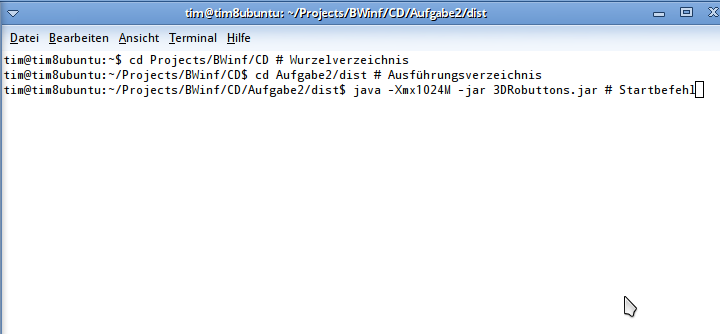
\includegraphics[width=\textwidth,height=.48\textwidth]{3d/1Konsole.png}
 \caption{Die drei Befehle um das Programm zu starten}
\end{figure}
\newline
Daraufhin öffnet sich der Startbildschirm.
Hier wird der Fenstermodus ausgewählt mit maximaler Auflösung (1280x720), um besser Screenshots machen zu können.
Also ist die Fullscreen-Auswahlbox nicht ausgewählt.
\begin{figure}[h]
 \centering
 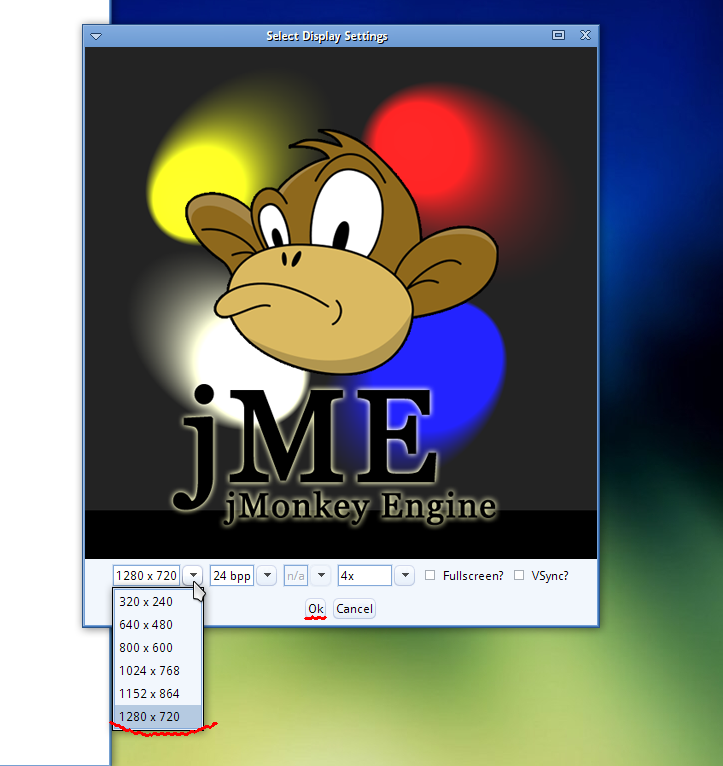
\includegraphics[width=.6\textwidth,height=.58\textwidth]{3d/2Aufloesung.png}
 \caption{Auswahl der Auflösung und Bestätigung per OK}
\end{figure}
\clearpage
\newpage
Nun öffnet sich das 3D-Fenster. Hier sind Robuttons blau, während Münzen als orange- bis bronzefarben zu erkennen sind.
\begin{figure}[h]
 \centering
 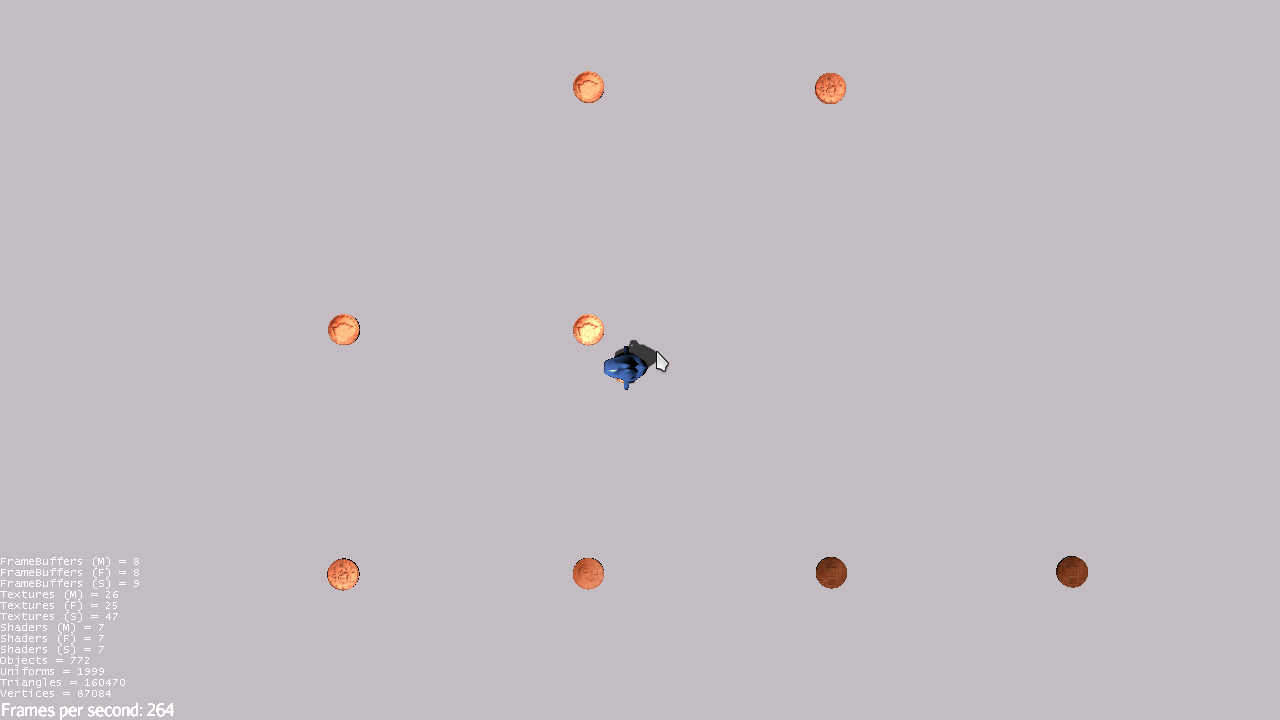
\includegraphics[width=\textwidth,height=.62\textwidth]{3d/2StandardAnsicht.png}
 \caption{Vor Start der Simulation, Standardansicht}
\end{figure}
\newline
Die Simulation wird nun mit der Leertaste gestartet, dann werden aus verschiedenen
Perspektiven und zu verschiedenen Zeitpunkten Screenshots gemacht.
Besonders spannend zu beobachten, ist das Abbauen von kleineren Haufen. Nach längerer Zeit bleiben in der Regel
nur wenige, größere Haufen übrig, da kleinere Haufen leichter abgebaut werden und Münzen nur an Haufen wieder
abgelegt werden. \\
Hier nicht zu beobachten, aber auch interessant: Wenn es so viele Robuttons gibt, dass alle Münzen
aufgenommen werden, dann sind nur noch Robuttons unterwegs und es bilden sich keine Haufen mehr, da
Münzen ohne andere, freiliegende Münzen nicht mehr abgelegt werden können.
\begin{figure}[ht]
 \centering
 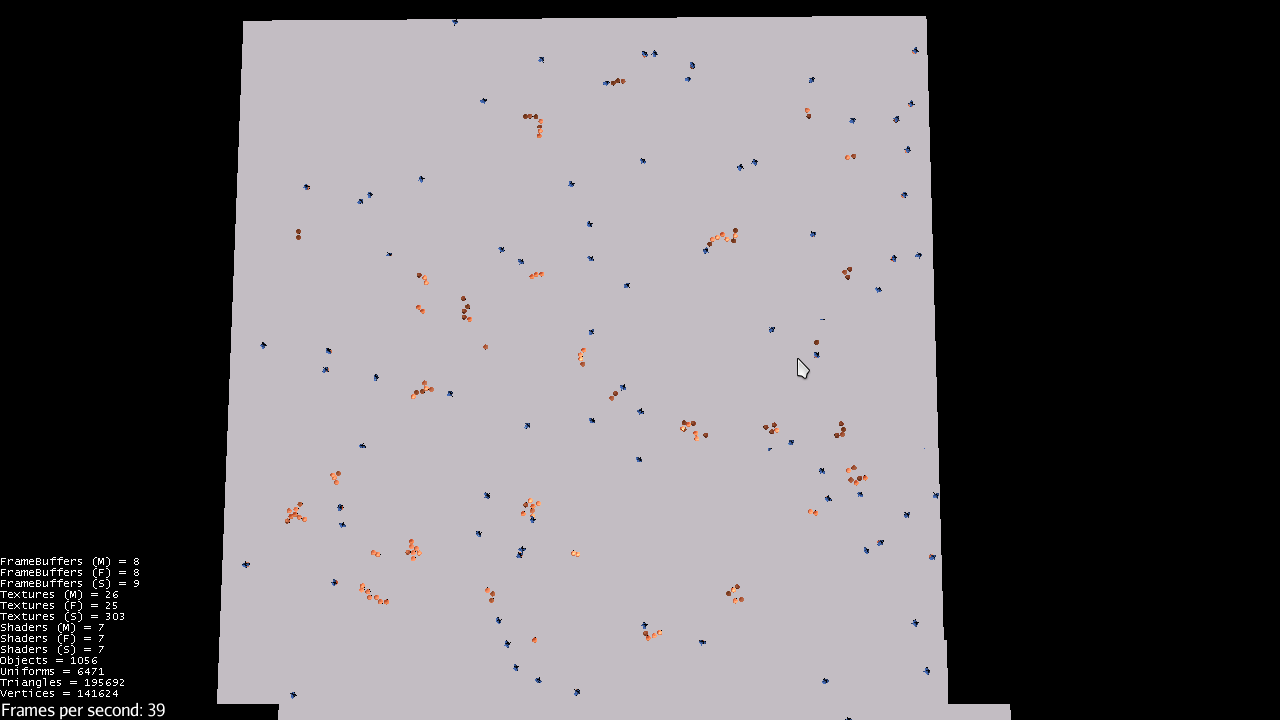
\includegraphics[width=\textwidth,height=.56\textwidth]{3d/3.png}
 \caption{Kurz nach Start der Simulation, bereits schwache Haufenbildung}
\end{figure}
\begin{figure}[ht]
 \centering
 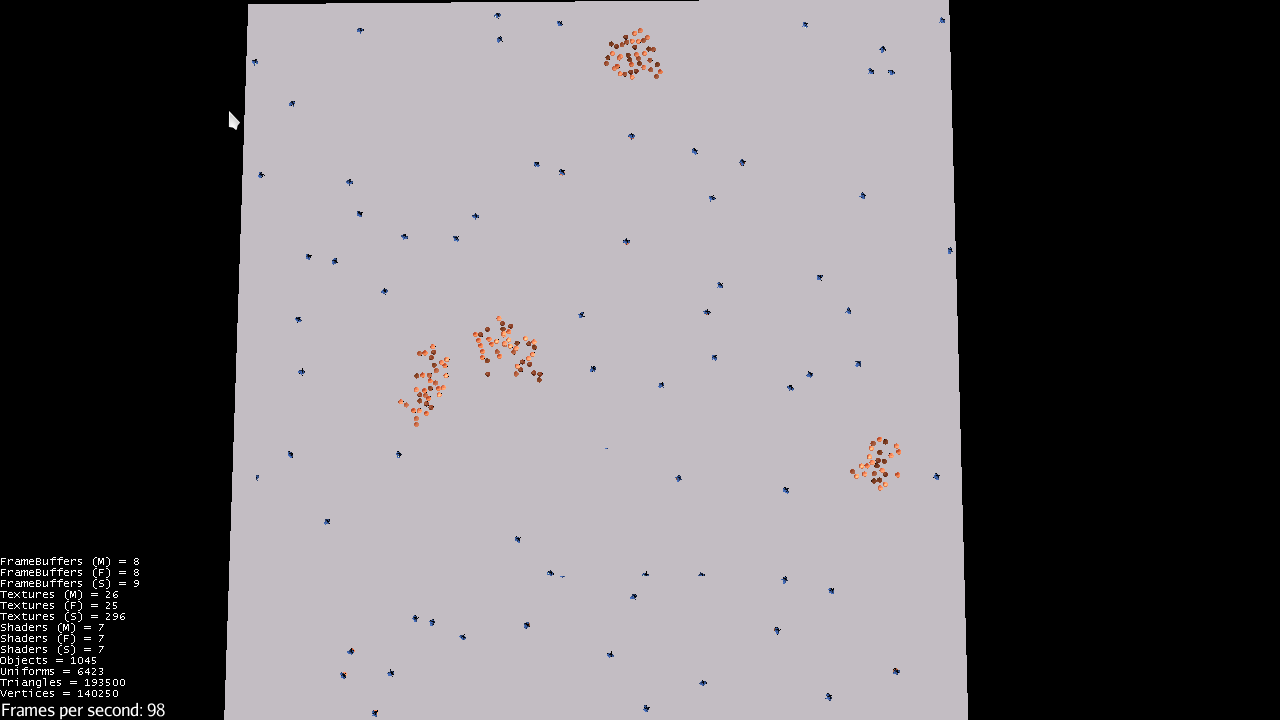
\includegraphics[width=\textwidth,height=.56\textwidth]{3d/3Haufen.png}
 \caption{Fortgeschrittene Simulation, nur noch vier große Haufen übrig}
\end{figure}
\begin{figure}[ht]
 \centering
 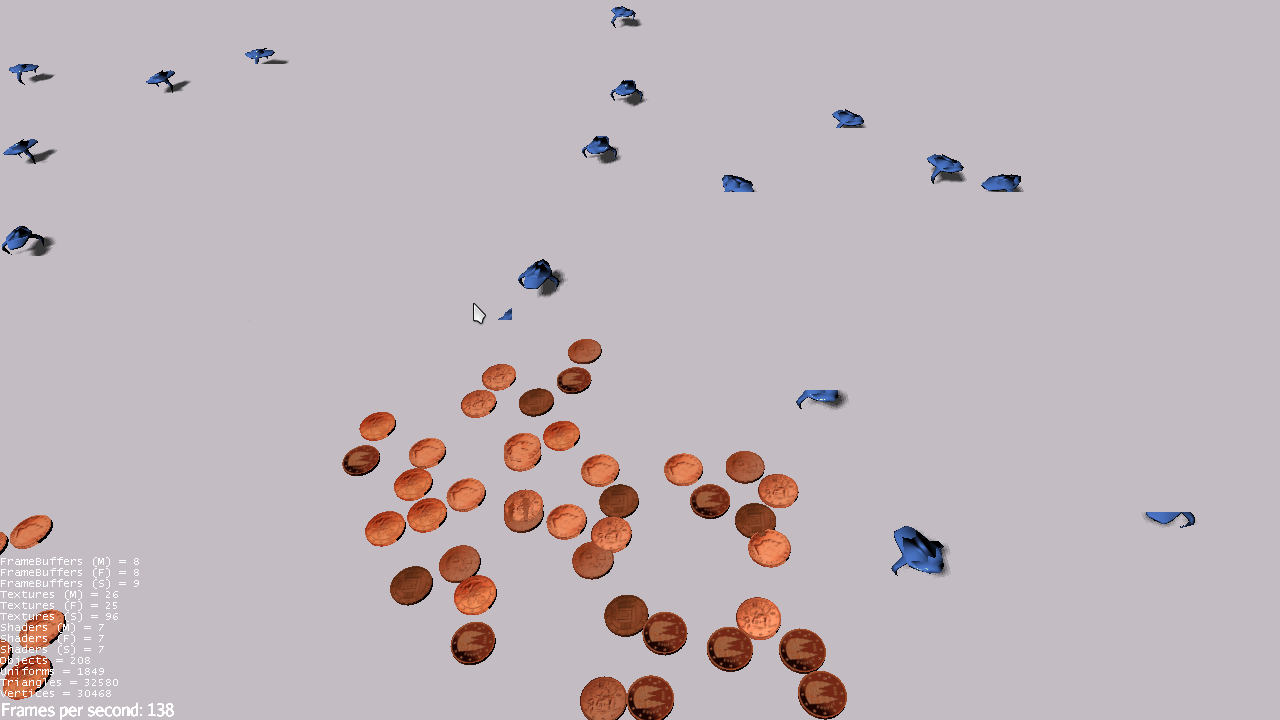
\includegraphics[width=\textwidth,height=.56\textwidth]{3d/Haufen_Nah.png}
 \caption{Einer der übriggebliebenen Haufen}
\end{figure}
\begin{figure}[ht]
 \centering
 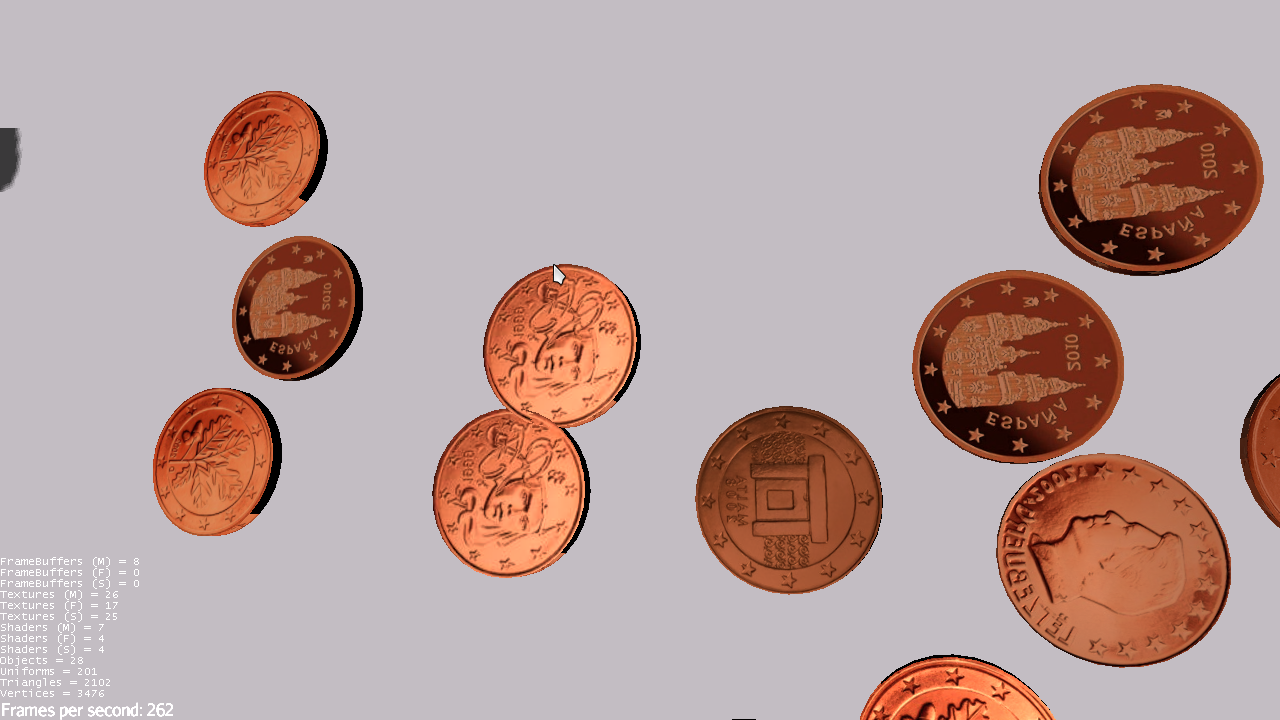
\includegraphics[width=\textwidth,height=.56\textwidth]{3d/Muenzen.png}
 \caption{5ct Münzen aus der Nähe}
\end{figure}
\clearpage\newpage
\subsection{Programm-Text}
Der Programm-Text ist wie folgt. Für das Multithreading ist einiger Zusatz-Code erforderlich.
Dieser konnte nicht ausgelassen werden, da er teilweise direkt die Logik implementiert.
\paragraph{Button.java:}
\lstset{language=Scala}
\lstset{basicstyle=\footnotesize}
\lstinputlisting{Button.java}
\paragraph{Robutton.java:}
\lstinputlisting{Robutton.java}
\paragraph{Coin.java:}
\lstinputlisting{Coin.java}
\paragraph{Table.java:}
\lstinputlisting{Table.java}
\paragraph{LineShape.java:}
Dies ist der Programm-Text, welcher die Kollisionserkennung in einem Tisch berechnet, gekürzt und vereinfacht.
\lstinputlisting{LineShape.java}
\subsection{Programm-Nutzung}
\paragraph{Systemvoraussetzungen:} (zusätzlich zu den allgemeinen Voraussetzungen, siehe \ref{Vor}):
Da bei diesem Programm Multithreading benutzt wird, sollte der Prozessor wenigstens 2 Kerne haben, um diese Funktion ausnutzen zu können.
Außerdem muss die Grafikkarte OpenGL2 implementieren, um die dreidimensionale Ansicht anzeigen zu können.
Eine möglichst hohe Rechenleistung der Grafikkarte, aber auch des Prozessors ermöglicht eine hohe Anzahl gleichzeitig simulierter Robuttons und Münzen.
\paragraph{Ausführung:}
Aufgrund von Beschränkungen durch die benutzte Engine, muss die Anwendung direkt im `dist' Verzeichnis ausgeführt werden.
Wechseln Sie daher zunächst aus dem Wurzelverzeichnis in das richtige Verzeichnis mit `cd Aufgabe2/dist'.
Die Ausführung erfolgt nun durch Eingabe des Befehles
`java -Djava.library.path=. -Xmx1024M -jar 3DRobuttons.jar' in der Konsole.\\
Es öffnet sich ein Fenster jME (jMonkeyEngine), in dem Sie aufgefordert sind, Ihre gewünschten Anzeigeeinstellungen anzugeben.
Empfohlen ist die Auswahl von Fullscreen und dann der maximalen Auflösung (z.B. 1280x720).
Wenn Sie einen langsameren Rechner haben, wählen Sie bitte eine niedrigere Auflösung.
Stellen Sie im 2. Feld ebenfalls den höchsten Wert ein (unter Windows ``32 bpp'', Linux/Unix ``24 bpp'').
Das Feld ``disabled'' bitte nicht verändern.
Nach Bestätigen mit OK öffnet sich ein weiteres Fenster mit 3D-Ansicht, in der Sie einen quadratischen Tisch mit Robuttons und Münzen sehen können.
\paragraph{Steuerung:}
Die Steuerung in der 3D-Ansicht, die sich öffnet, ist folgende: \\
\begin{center}
\begin{tabular}{ll}
\textsc{Steuerung} & \textsc{Eingabemethode, z.B. Taste} \\
\hline\hline
Simulationsstart & Leertaste \\
Kamera Hoch/Runter & Tasten W/S \\
Kamera Links/Rechts & Tasten A/D \\
Kamera-Rotation & Maus hoch/runter, links/rechts für Rotation um die Kameraachsen \\
Kamera-Zoom & Mausrad \\
Simulationsende & Esc (oder zur Not Alt+F4)
\end{tabular}
\end{center}
